% TEX encoding = UTF-8 Unicode
% Complied by LaTeX, not XeLaTeX
% if documents are needed, using BibTeX first after aux file generated.

\documentclass[12pt, oneside]{article}   	
\usepackage{geometry}                		% See geometry.pdf to learn the layout options. There are lots.
\geometry{a4paper}                   		% letterpaper or a4paper or a5paper or ... 
\usepackage{graphicx}				% Use pdf, png, jpg ...
\usepackage{caption}
\usepackage{subcaption}
\usepackage{amssymb}				% Math package
\usepackage{CJKutf8}				% set Chinese support
\usepackage{indentfirst}				% Keep 2 space indent at the begin of a new chapter.
\usepackage{setspace}				% set line space
\usepackage{amsmath}				% Math package, like align
\usepackage{bbm}					% use indicator function in math

\title{微博情绪分析}
\author{
	Yuxin Chen\\
	\texttt{13307130xxx}
	\and
	Yimu Wan\\
	\texttt{13307130xxx}
	\and
	Yong Xu\\
	\texttt{12307130xxx}
	\and
	Shumin Wang\\
	\texttt{12307130xxx}
}
\date{\today}

\begin{document}
\begin{spacing}{1.5}
\begin{CJK}{UTF8}{gbsn}

\maketitle

% \tableofcontents

\newpage

\section{介绍}

\section{结果}
\subsection{微博量-时间}
\label{subsec:weibo_time}
在这一小节中我们统计了微博量与时间的关系。程序实现中,首先将每一条微博 map 为 {\it(HH:MM, emotion)} 的 key-value pair,其中 HH:MM 表示小时和分钟数, emotion 表示情绪(这里复用了\ref{subsec:emotion_time}节中的程序)。再对 map 好的 key-value pair 根据键的值来做 reduce 。 

图\ref{fig:weibo_time}展示了以小时为间隔的统计结果。数据显示,9时-24时微博量相对稳定,高峰出现在22时-23时这一区间内。23时之后微博量开始下降,低谷在5时-6时出现,呈现一个明显的U形,符合大部分人的作息习惯。

\begin{figure}
	\centering
	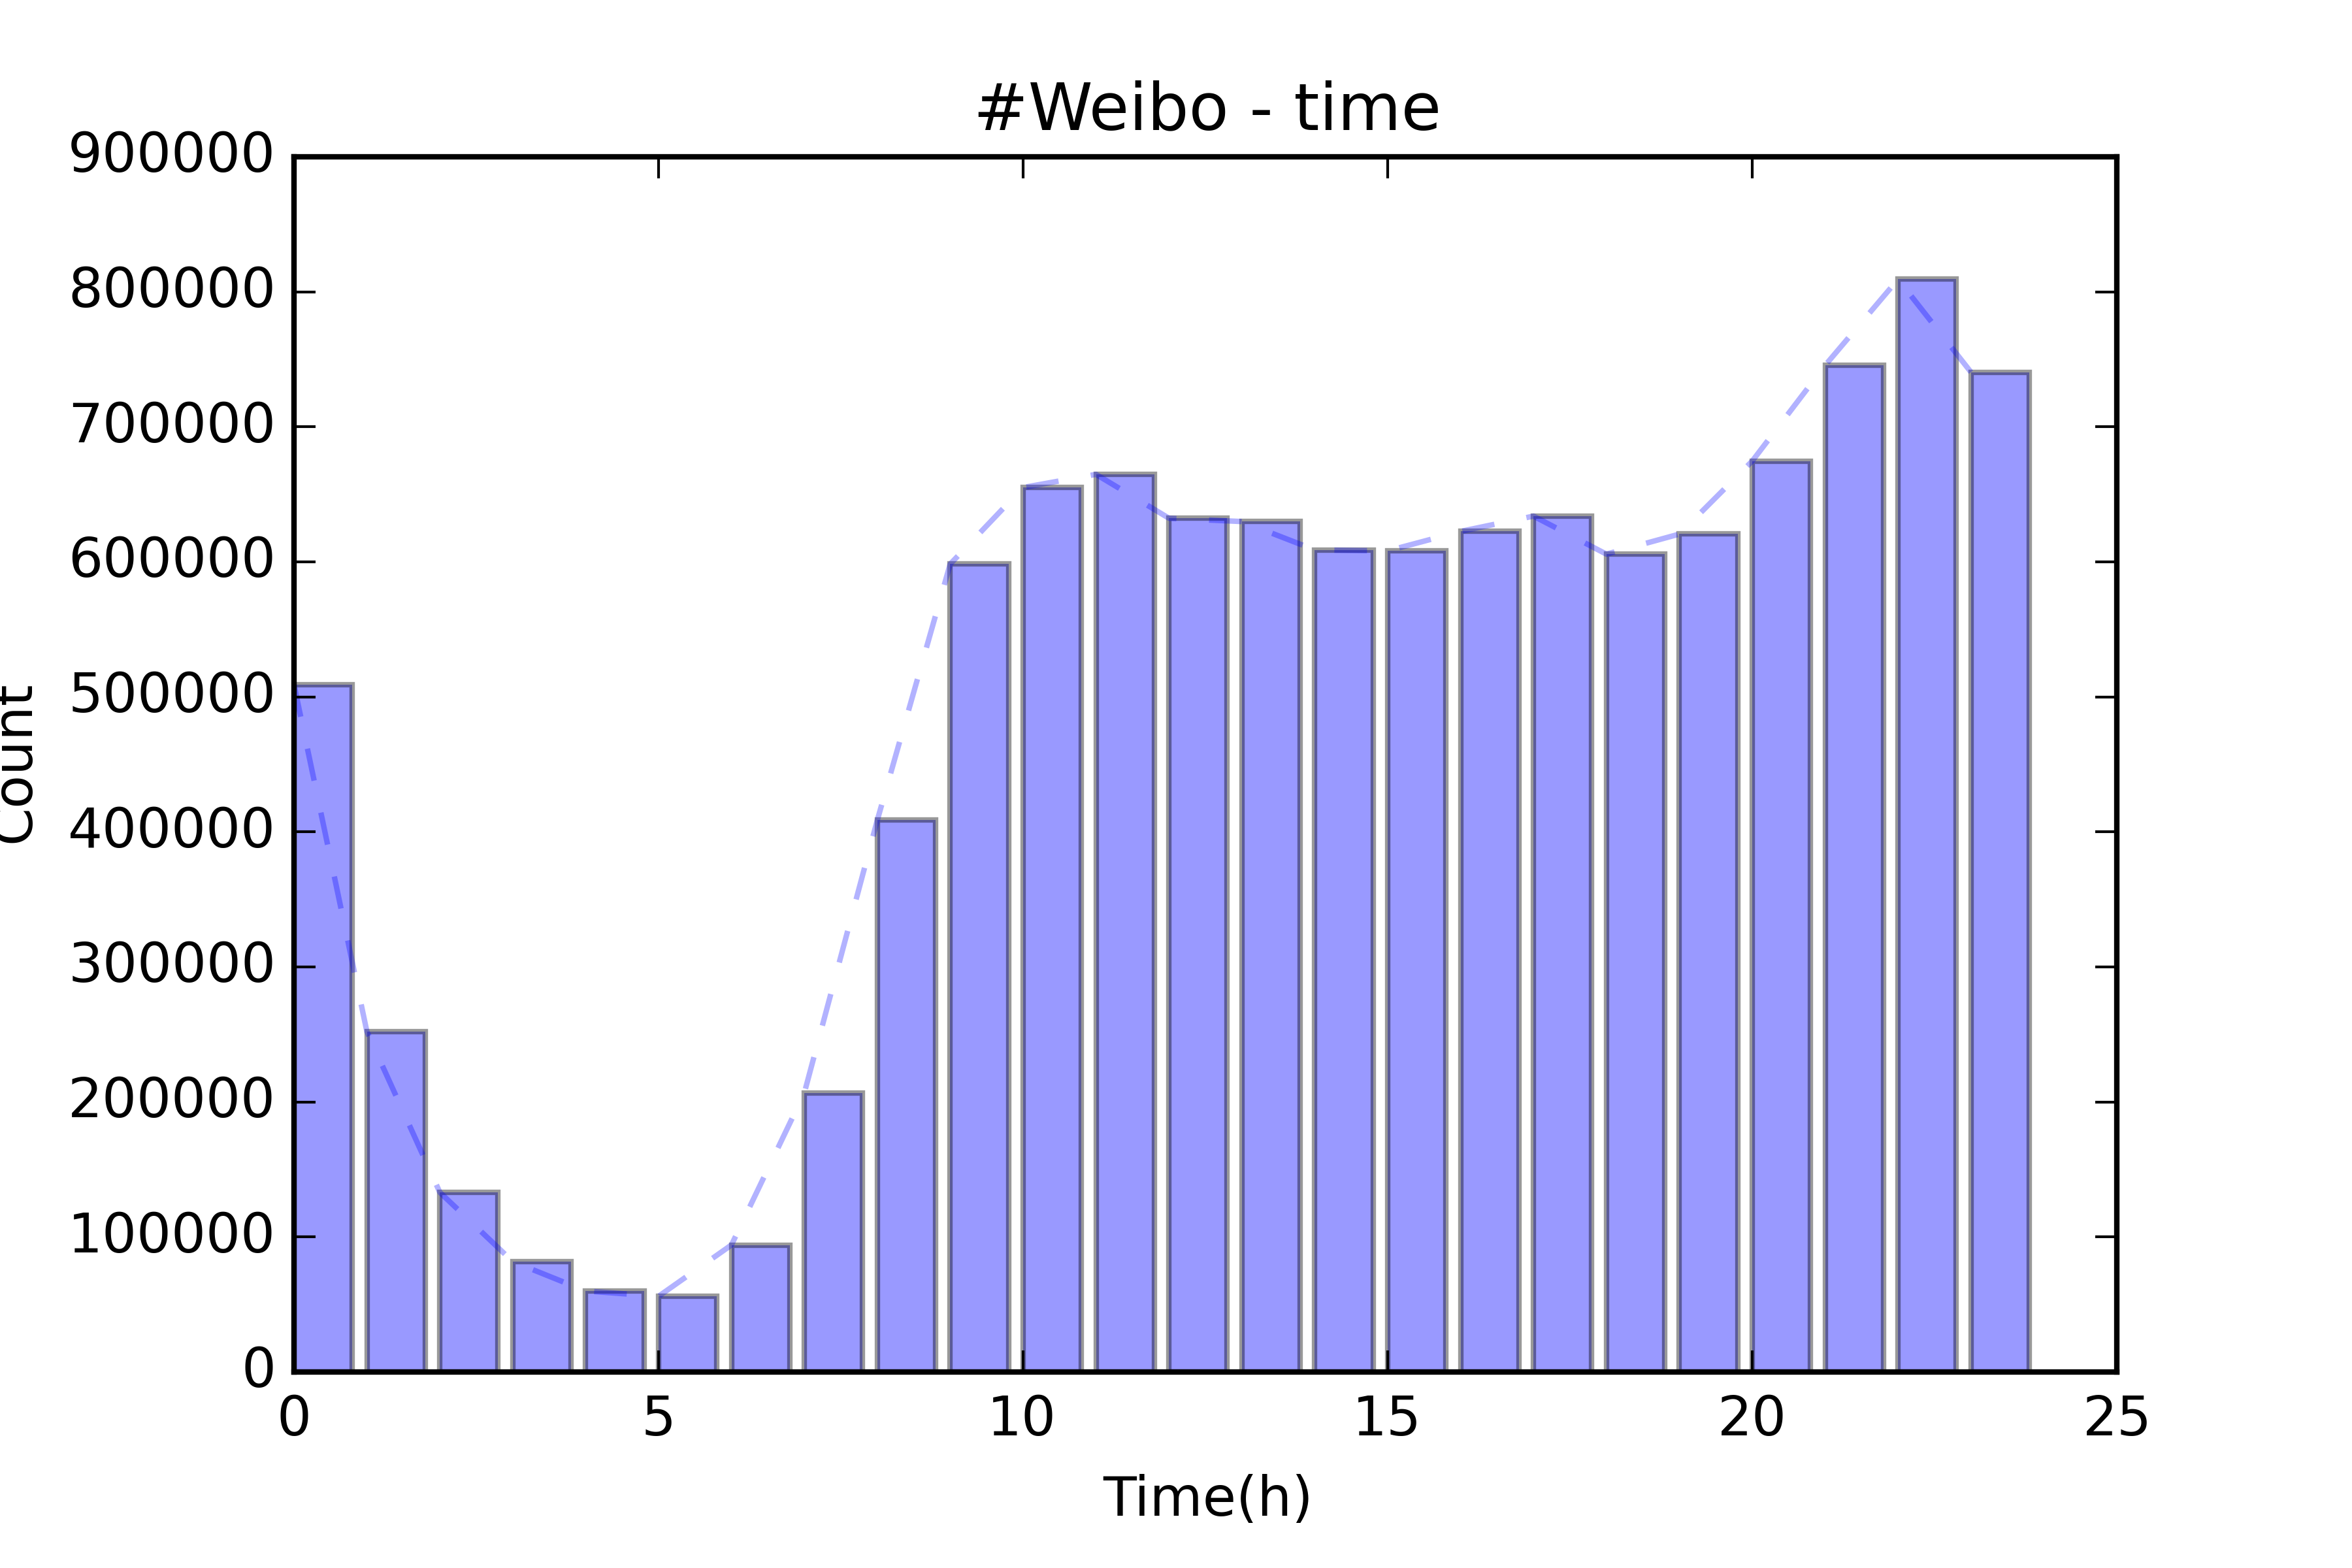
\includegraphics[width=0.8\linewidth]{../result/charts/weibo_time}
	\caption{微博量-时间}
	\label{fig:weibo_time}
\end{figure}

\subsection{微博情绪-时间}
\label{subsec:emotion_time}
在这一节中我们试图通过统计来揭示微博情绪随时间的变化情况。程序实现中,map和reduce操作在\ref{subsec:weibo_time}节中已经介绍,这里补充说明 {\it(HH:MM, emotion)} 的 key-value pair 中 emotion 的计算方法。计算方法如下:
$$
emotion = 
\begin{cases}
1 & npos > 0~and~nneg = 0 \\
-1 & npos = 0~and~nneg > 0 \\
2 & nneg > 0~and~npos >= nneg \\
-2 & npos > 0~and~nneg > npos \\
0 & \text{otherwise}
\end{cases}
$$
公式中的 {\it npos, npeg} 为预处理后统计出来的两个数值,代表微博中包含的正负表情个数。 公式的结果中,1和-1代表这条微博具有明显的情绪倾向,0代表微博中不包含含有情绪的表情(或者表情不在数据集的情感词典中出现),2和-2代表这条微博的情绪有歧义,但更偏向积极或更偏向消极。

图\ref{fig:emotion_time_1}反映了有明确情绪的微博和总微博数量之间的关系。没有明确情绪的微博由上述 emotion 为 0和±2的微博组成。图\ref{fig:emotion_time_2}反映了积极微博和消极微博数量上的关系,可以明显的看出,情感积极的微博总是占据大多数的。为了更好的体现微博整体情感的变化趋势,我们使用 {\it PN ratio} 来衡量整个微博的情感。
$$PN~ratio = \frac{\text{\#positive weibo}}{\text{\#negative weibo}}$$
图\ref{fig:emotion_time_3}反映了 {\it PN ratio} 与时间的关系。有意思的是,整体的图形与微博量-时间的图形非常相似,这也就意味着,在深夜的时候,消极微博占的比重更大。

\begin{figure}
	\centering
	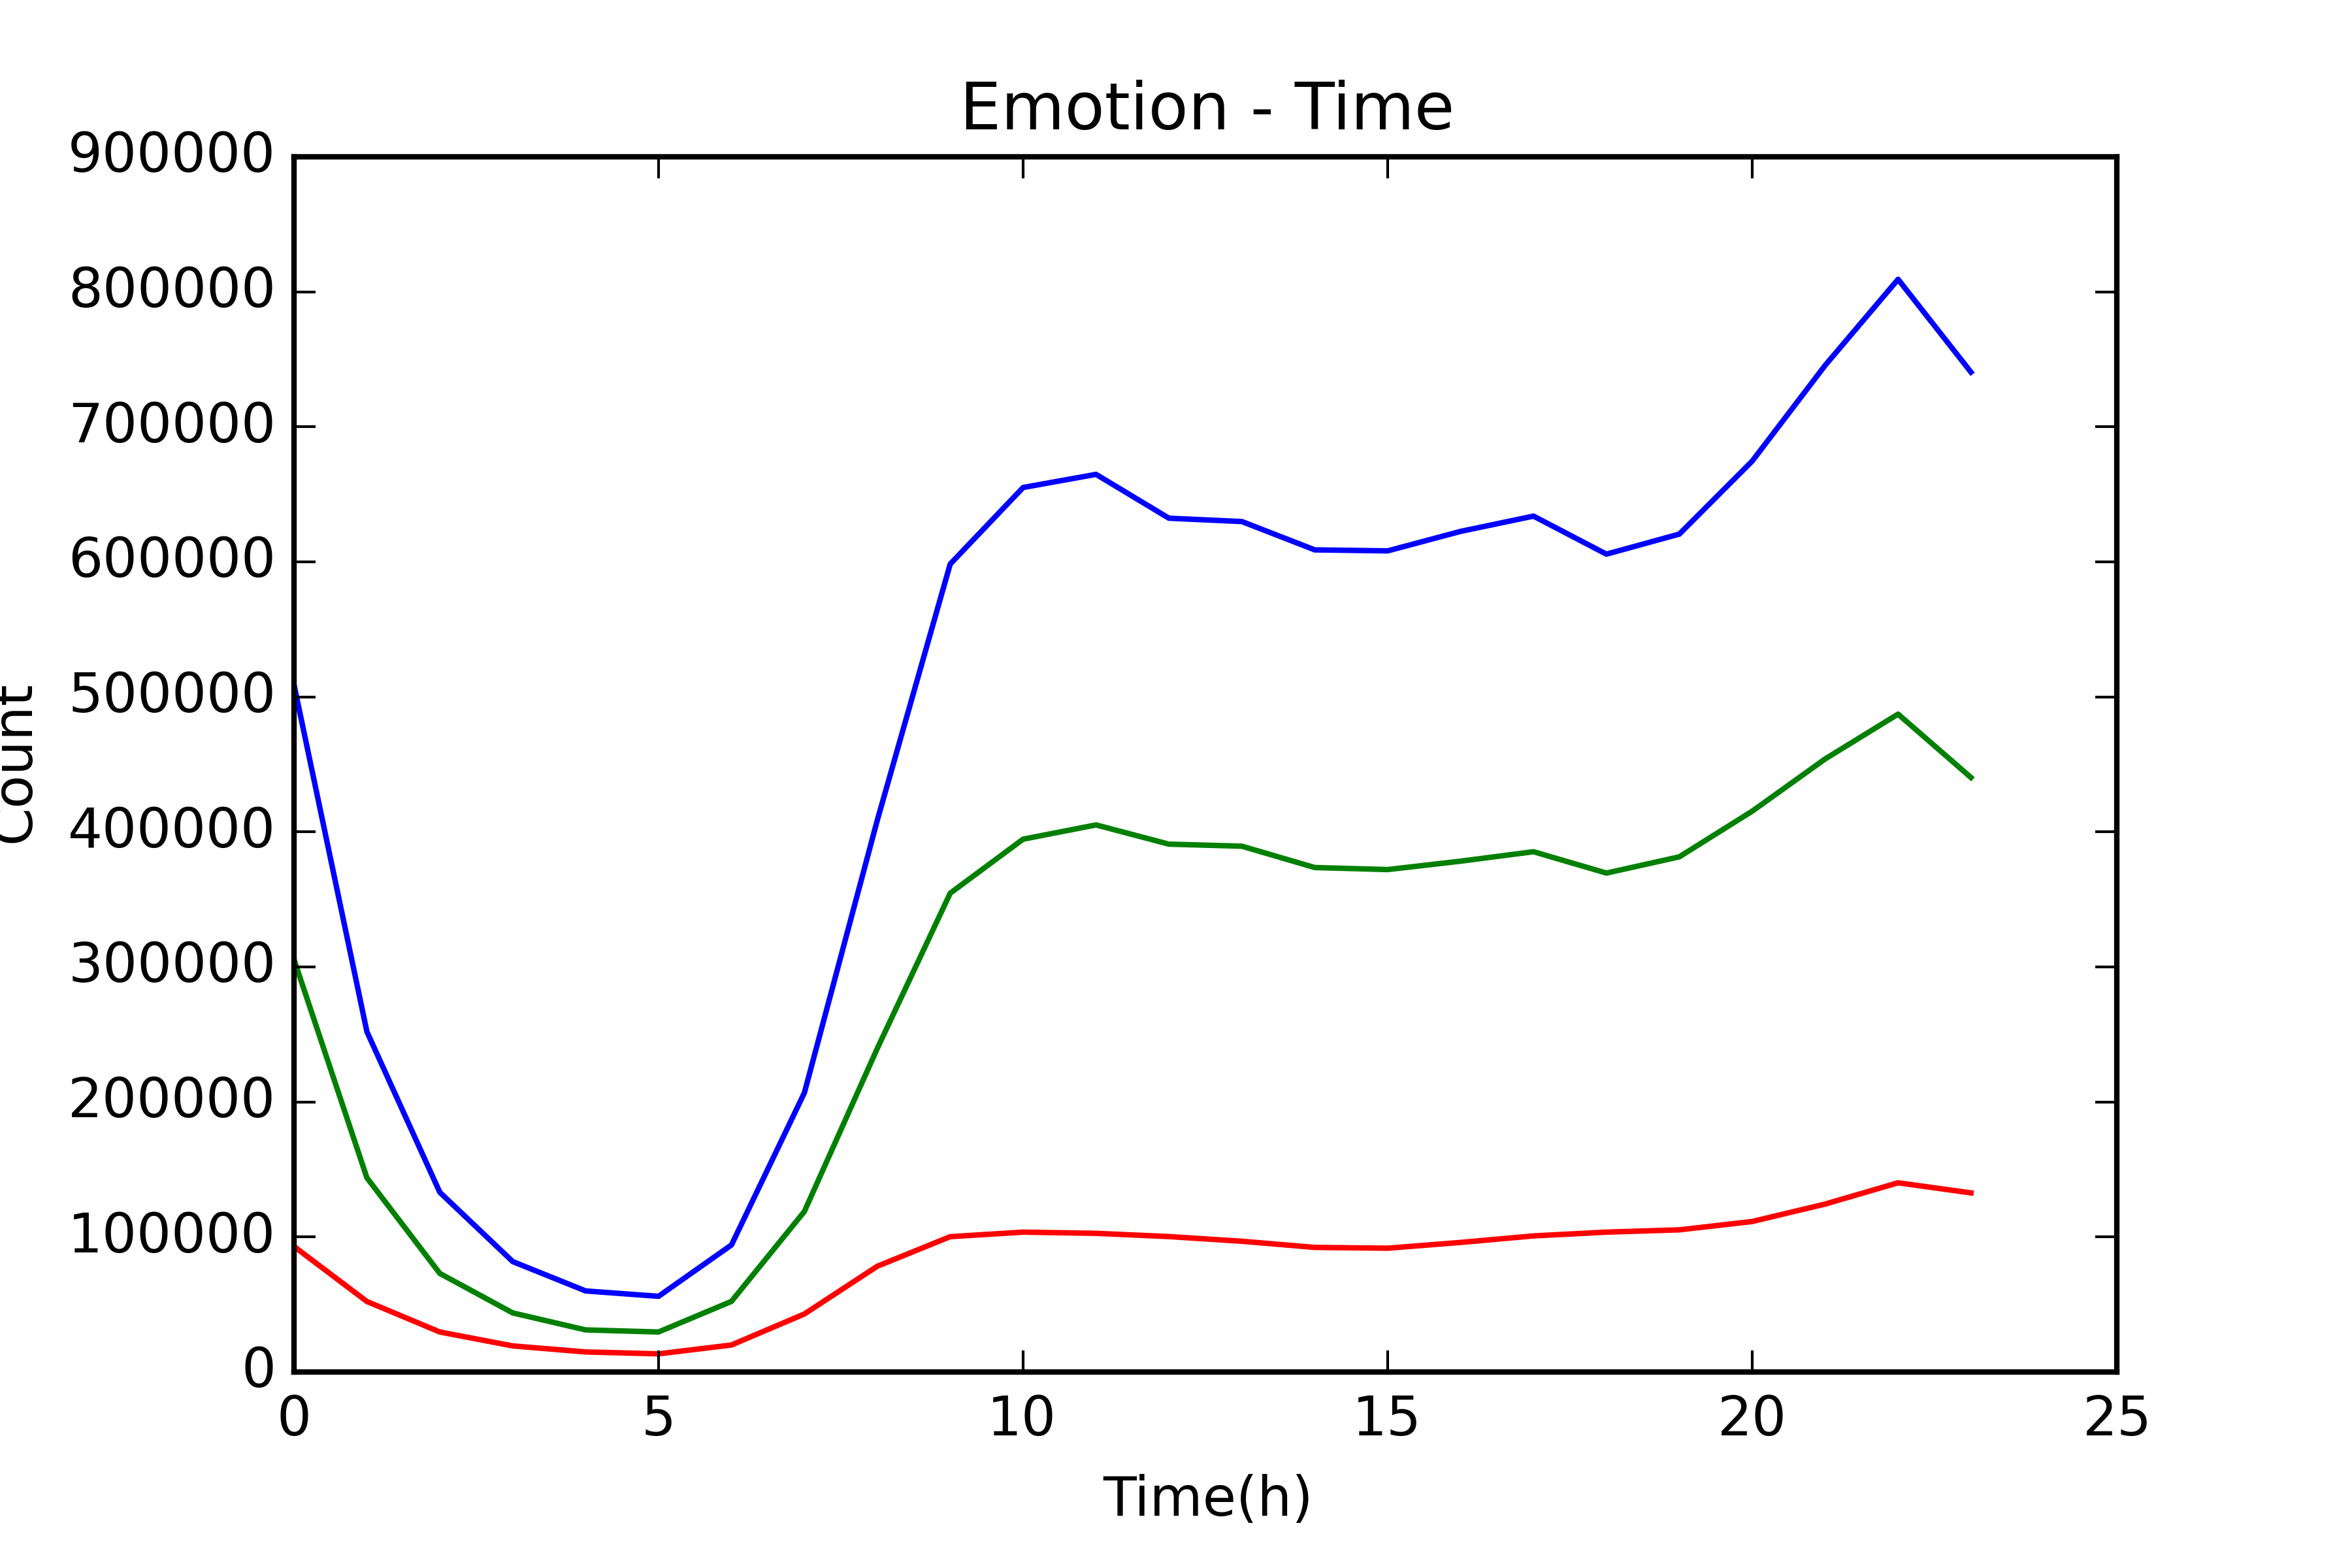
\includegraphics[width=0.8\linewidth]{../result/charts/emotion_time_1}
	\caption{有明确微博和总微博数量的关系。图中绿色线表示所有微博量,蓝色为积极情绪,红色为消极情绪。}
	\label{fig:emotion_time_1}
\end{figure}
\begin{figure}
	\centering
	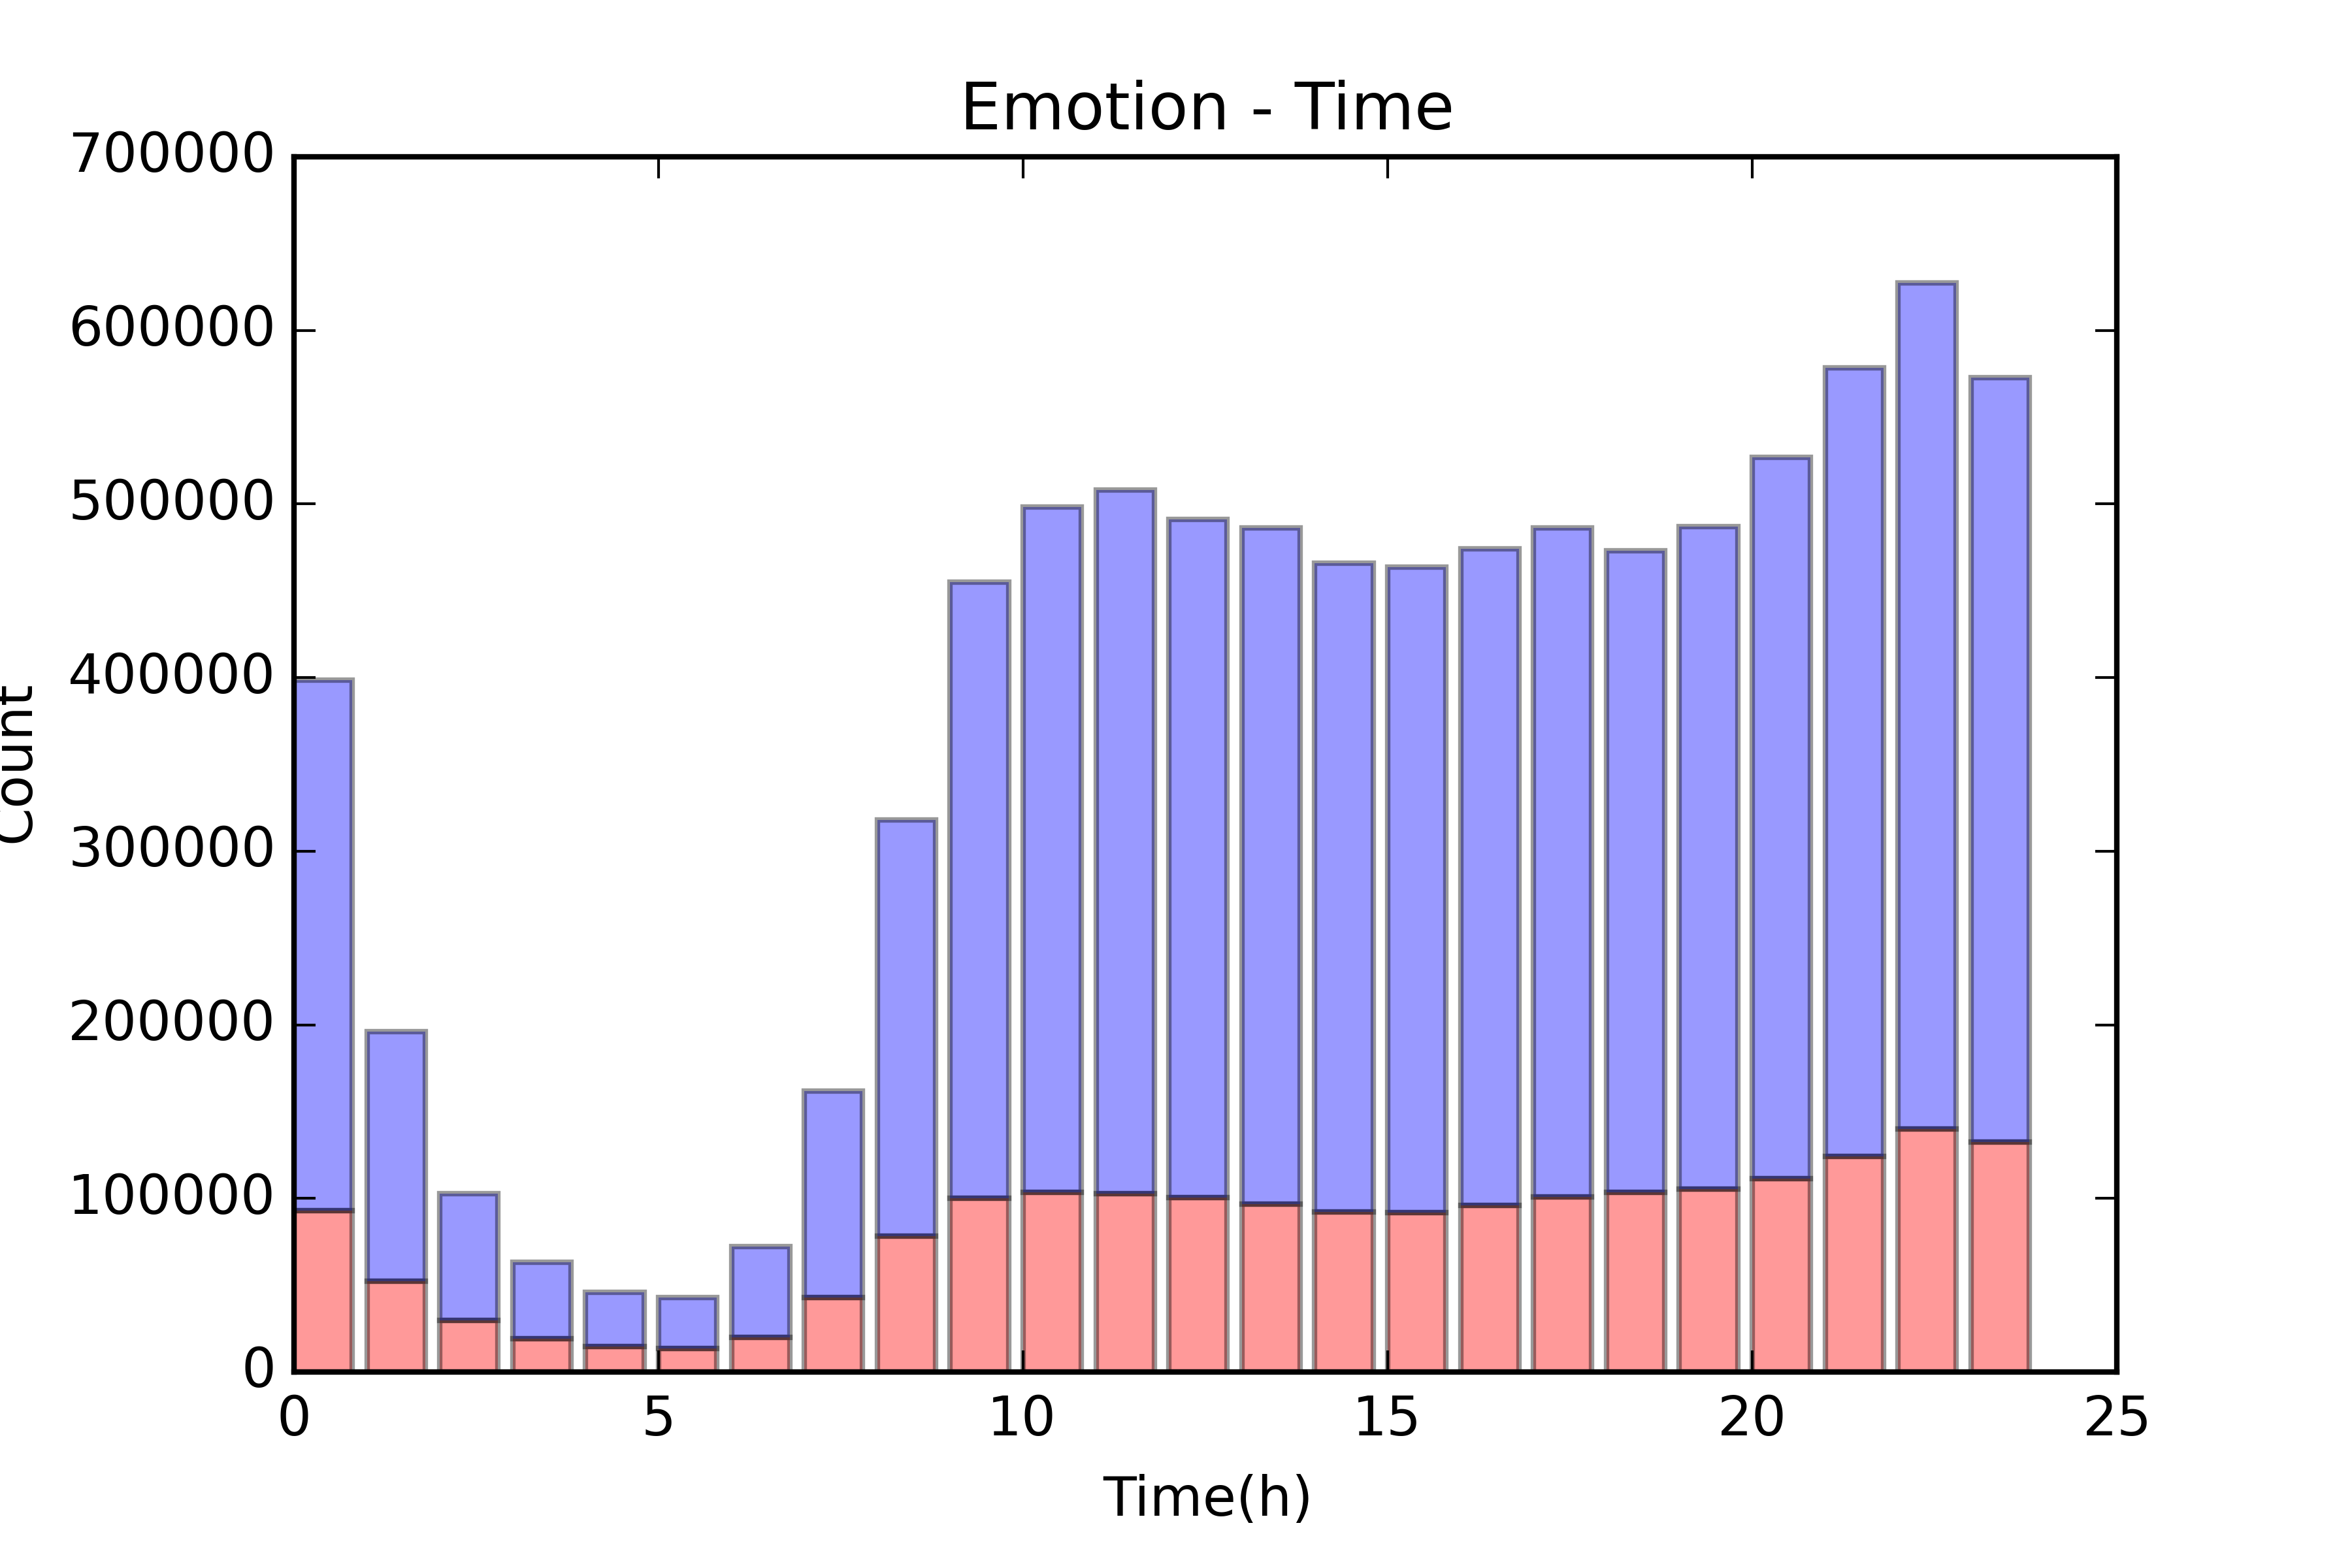
\includegraphics[width=0.8\linewidth]{../result/charts/emotion_time_2}
	\caption{微博情绪-时间(不包括没有明确情绪的微博)。图中蓝色代表积极情绪,红色代表消极情绪,蓝色柱堆叠于红色柱上方。}
	\label{fig:emotion_time_2}
\end{figure}
\begin{figure}
	\centering
	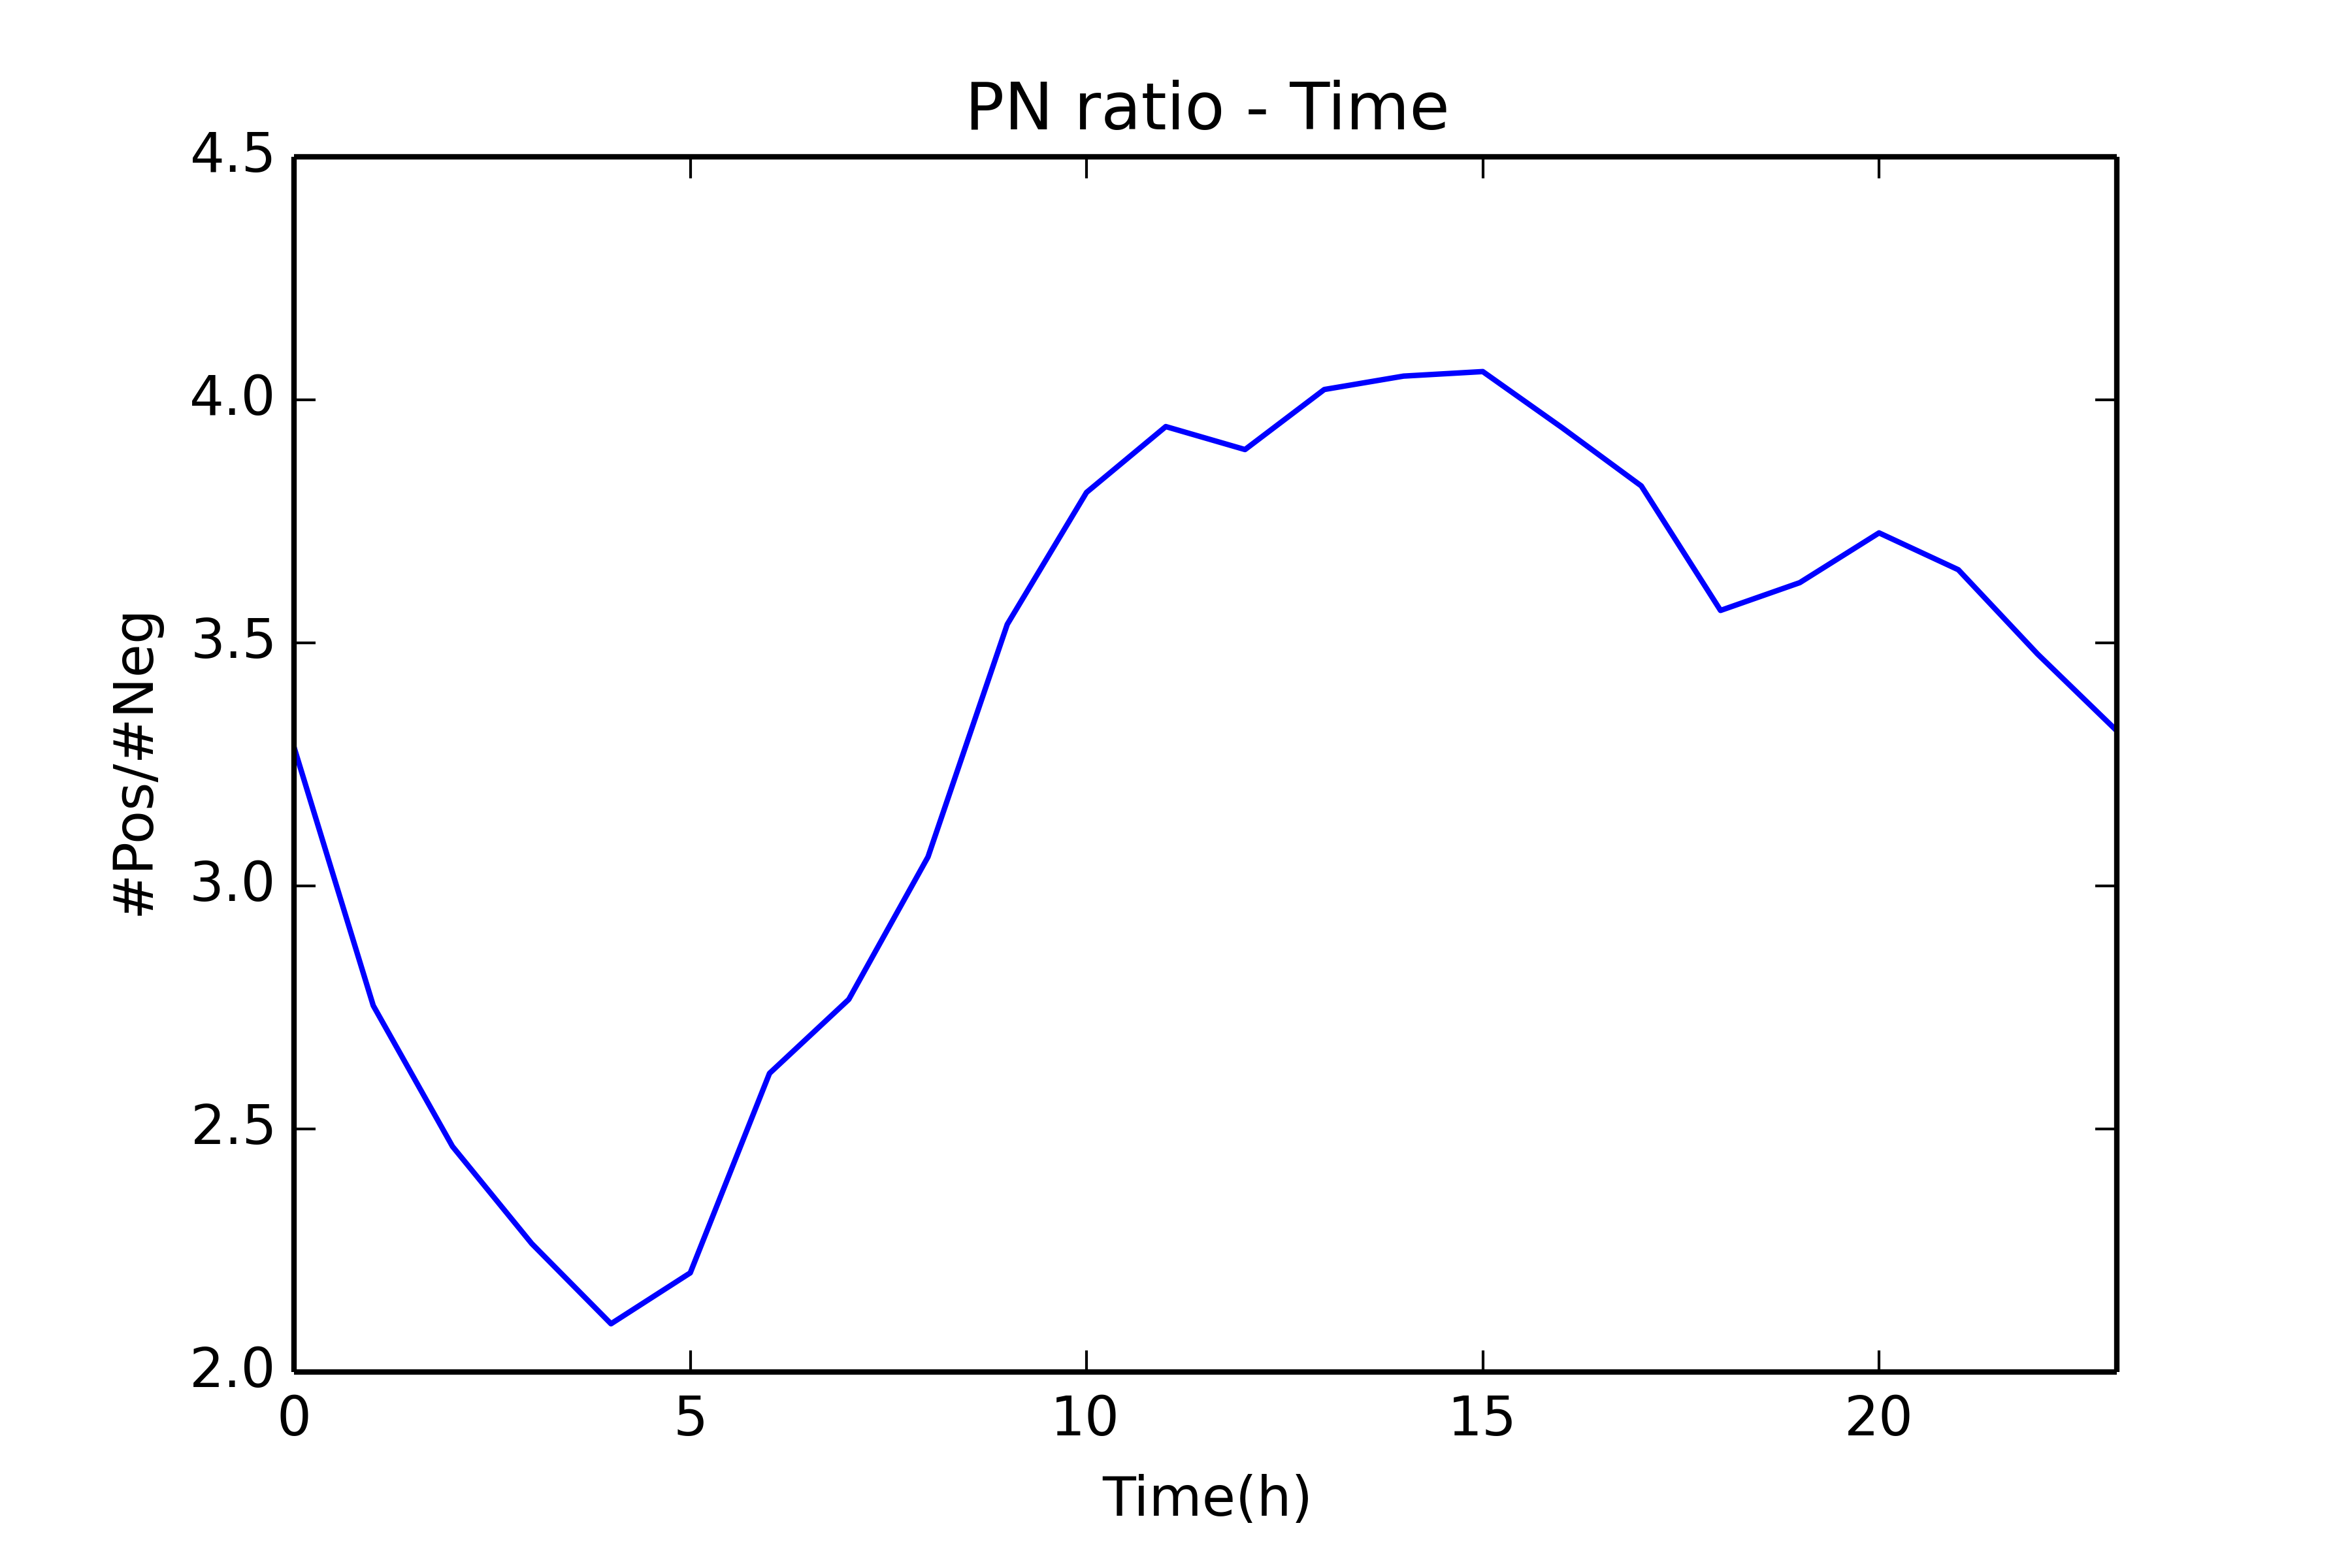
\includegraphics[width=0.8\linewidth]{../result/charts/emotion_time_3}
	\caption{积极与消极微博比例和时间的关系。}
	\label{fig:emotion_time_3}
\end{figure}

\subsection{微博情绪-日期}
这一小节我们分析每日微博情绪(使用 {\it PN ratio} 衡量)波动,并以此检验衡量标准是否有效。从\cite{bollen2011twitter}中作者的实验来看,好的衡量标准应该能够准确的反映重大公众事件的发生。因此我们在实验之前,预期 {\it PN ratio} 在春节等节日应该达到最大,在5·12等纪念日时达到低谷。

实验结果符合我们的预期, {\it PN ratio} 能够如实体现重大公众事件发生后大众心理的变化。积极情绪中:2012年01月01日,元旦,微博情绪达到了全年最高峰, {\it PN ratio} 为5.87。2012年01月22日,除夕,{\it PN ratio} 达到了另一个极大值5.76。随后的大年初一,该值仍维持较高的水平,达到5.51。到了2012年01月28日,春节7天假期结束,上班族不得不重返工作岗位,微博相应的出现了较多的消极情绪,这一天 {\it PN ratio} 为2.96。全年还有两个明显的峰值,一个是在2012年02月14日的情人节,另一个则是在2012年06月01日的六一儿童节。

消极情绪方面:2012年05月12日,汶川大地震四周年,微博上包括名人、机构在内的众多网友纷纷发微博表示悼念, {\it PN ratio} 为2.29。此外,2012年07月22日和2012年07月23日两天达到了全年的最低谷, {\it PN ratio} 分别为2.09和2.19。经过采样分析,主要与两件事情有关,一是2012年07月22日重创北京的大暴雨,二是2011年7月23日发生的甬台温铁路列车追尾事故。两件事情的叠加,使得微博上出现了更多悼念和问责的声音,最终把情绪拉向了全年的最低谷。初次之外,2012年01月28日还出现了一次低谷,{\it PN ratio} 为2.96,经过分析,与惠特尼·休斯顿去世有关。通过数据还可以类似的找出其于公众事件的关联,在此不再赘述。

\begin{figure}
	\centering
	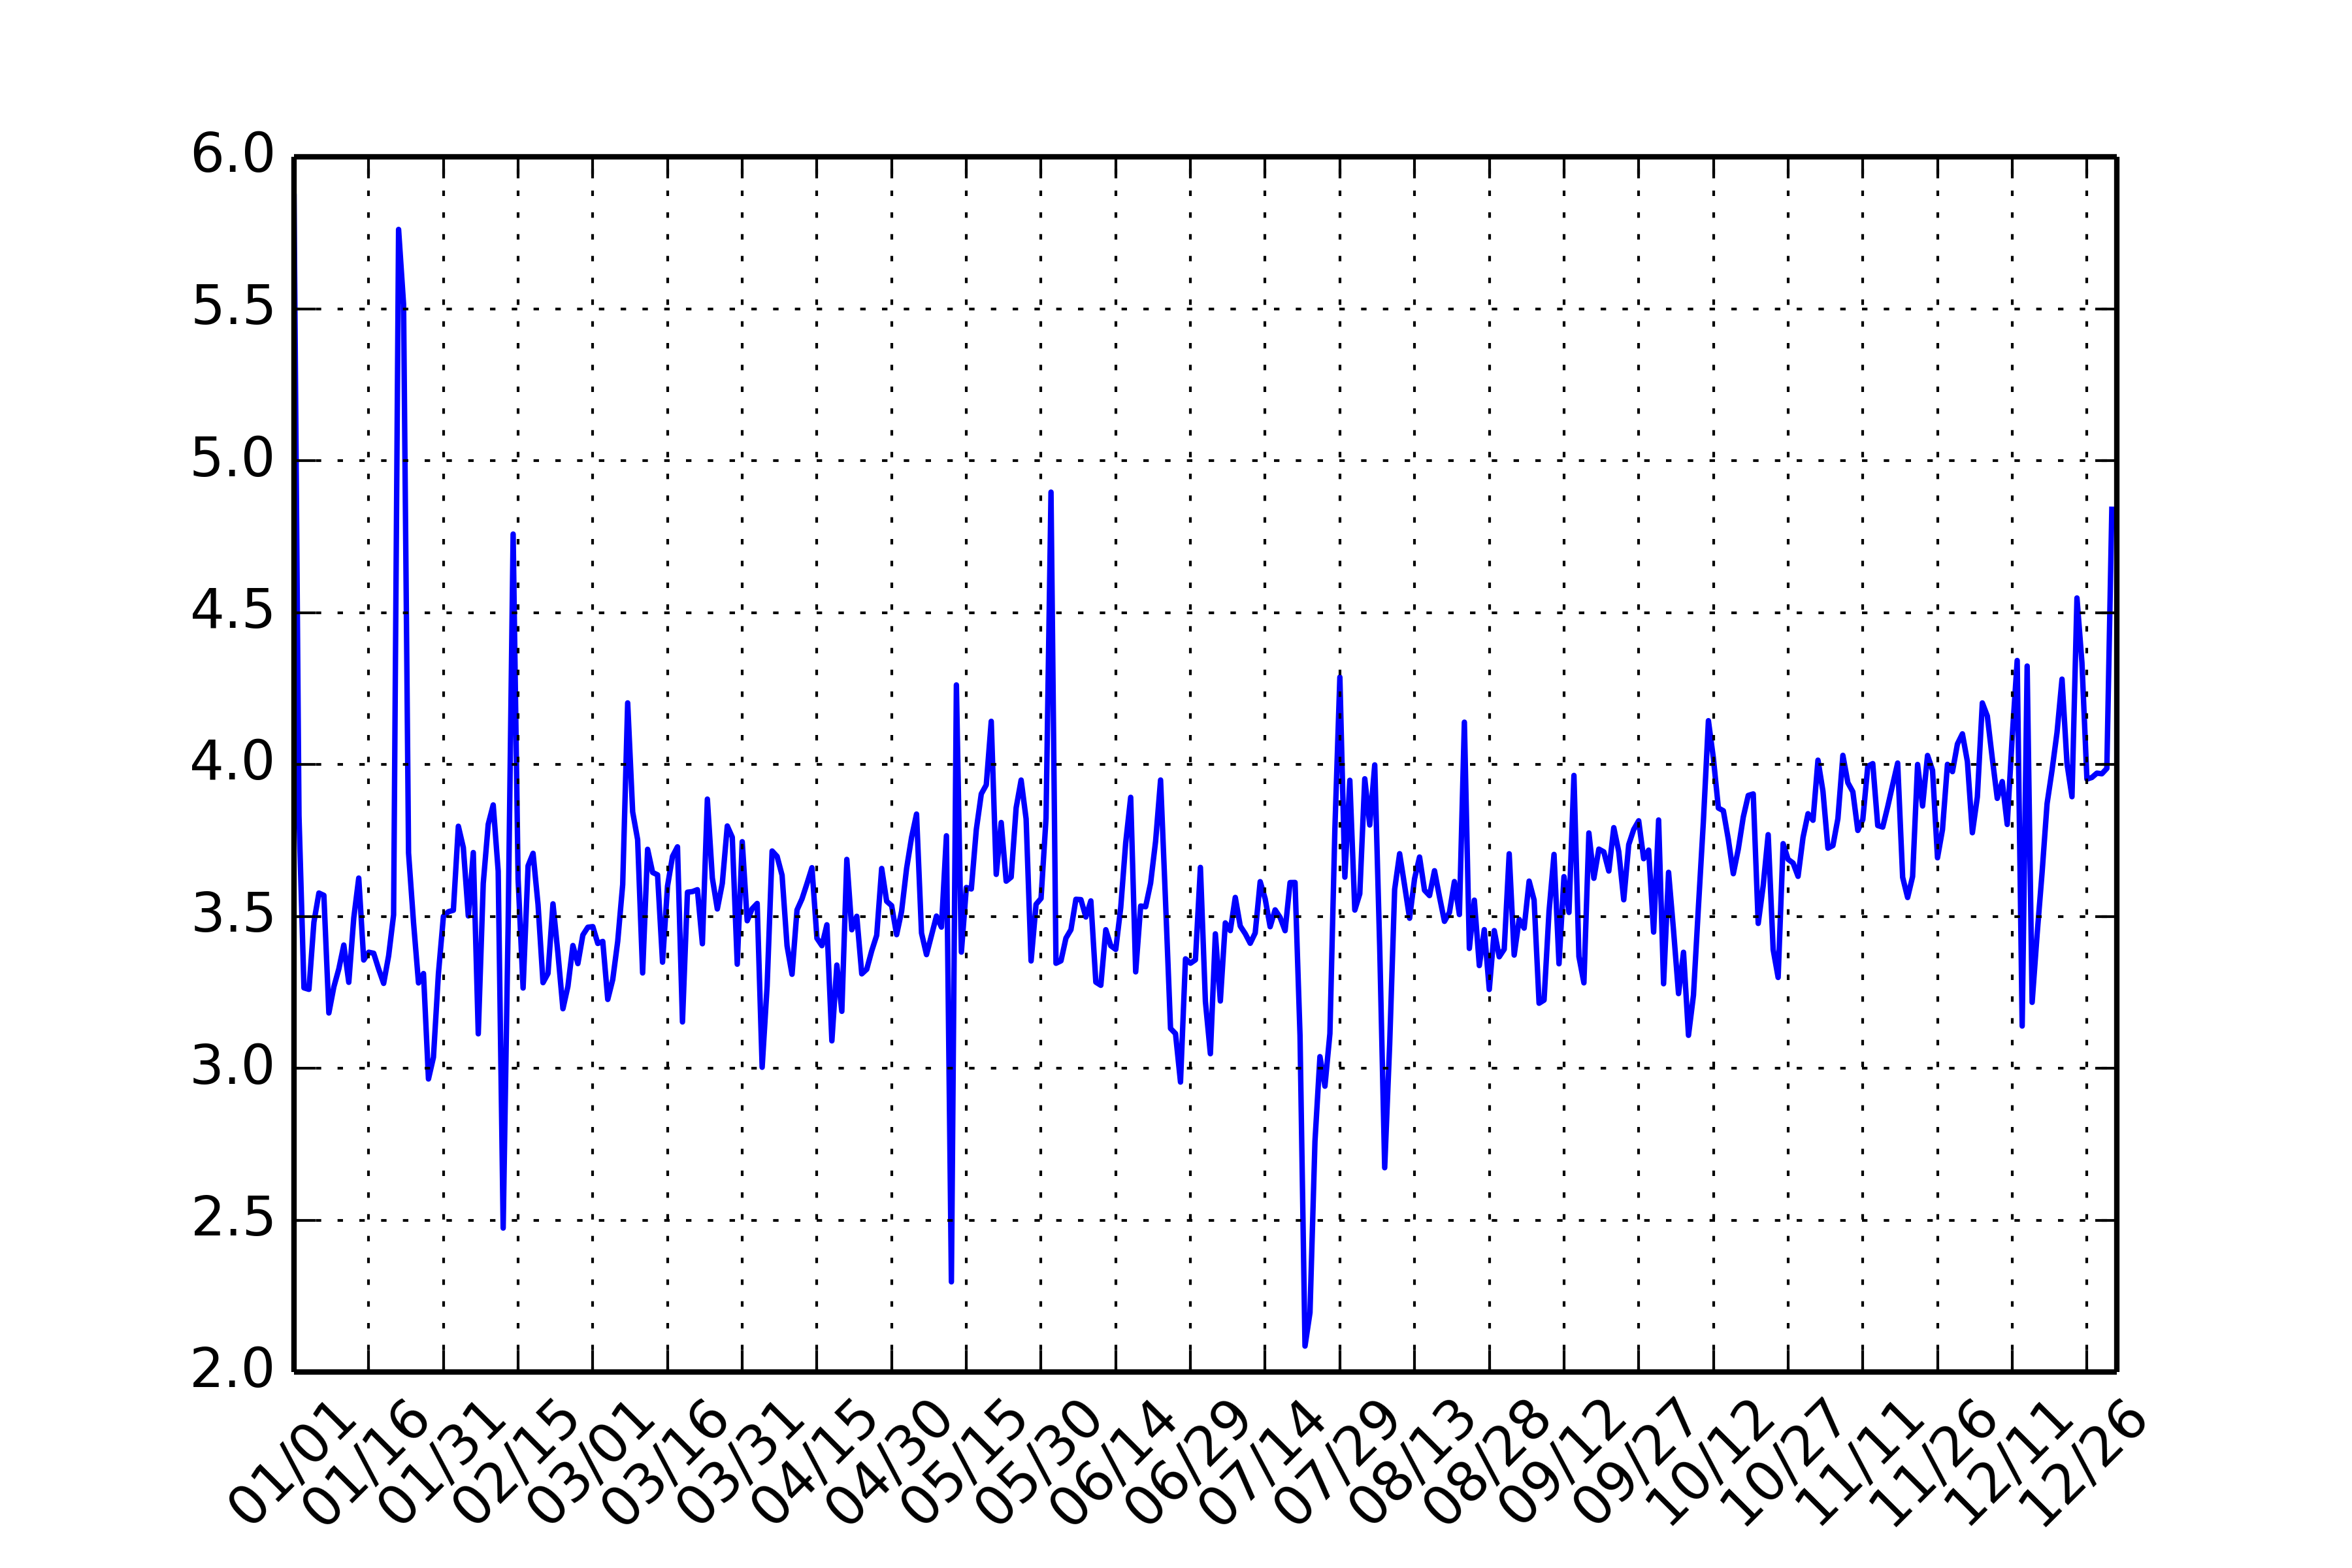
\includegraphics[width=0.8\linewidth]{../result/charts/emotion_day}
	\caption{2012年日微博情绪波动。}
	\label{fig:emotion_day}
\end{figure}

\newpage
\renewcommand\refname{参考文献}
\bibliographystyle{plain}
\bibliography{Report}

\end{CJK}
\end{spacing}
\end{document}
